\documentclass{beamer}
\usetheme{Madrid}
%\usetheme{Berlin}
%\usepackage{german}
%\usepackage[latin1]{inputenc}
%\usepackage[T1]{fontenc}
\usepackage{hyperref}
\usepackage{booktabs}
\usepackage{graphicx}
\usepackage{epsfig}
\usepackage{listings}
\usepackage{array}
\usepackage{colortbl}
\usepackage{changebar}
\usepackage{amsmath}
\usepackage[T1]{fontenc}
%\usepackage[ansinew]{inputenc}
\usepackage{setspace}
\usepackage{multicol}
\usepackage{dcolumn}
\usepackage{color}
\usepackage{wasysym}
\usepackage{movie15}
\usepackage{MnSymbol}
\usepackage{marvosym}
\usepackage{pifont}
%\usepackage[table]{xcolor} 
%\beamerdefaultoverlayspecification{<+->}
\setbeamertemplate{footline}%{infolines theme}



\begin{document}

\lstset{
basicstyle=\ttfamily,
keywordstyle=\bfseries,
showstringspaces=false,
columns = fullflexible,
mathescape = false,
language=R
}


\title[Gallop Network Formation]
{PS 632: Solving Endogeneous Networks Computationally}
\author[M. Gallop]
{Max Gallop} 
\institute
{		Department of Political Science\\
		Duke University\\
		
		}

\date{Version 1.0}

\begin{frame}
\titlepage
\end{frame}

\begin{frame}{Approximately 70\% of Social Network Presentations\footnote{May be an exaggeration}: Featuring this Class}
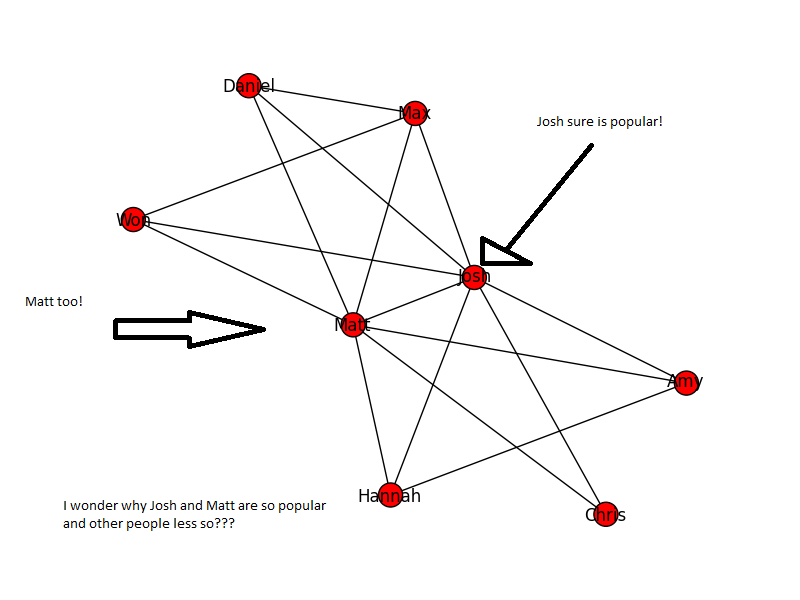
\includegraphics[scale = .5]{StupidExample.png}
\end{frame}


%\begin{frame}{The Issue}
%\begin{itemize}
%\item People love Social Network Analysis.
%\item And its in many ways a better way to conceptualize phenomena that we care about in the social sciences, since it accounts for interdependencies.
%\item Yet, the SNA currently in use is significantly more primitive than using basically every other methodology generally falling into one of three categories:
%\begin{enumerate}
%\item Basic description of a network.
%\item More complicated description of a network (using latent space or random graphs to account for uncertainty in observing a network).
%\item Naively using some characteristic of a graph as a right hand variable in regression.
%\end{enumerate}
%\end{itemize}
%\end{frame}

\begin{frame}{A Particular Issue with SNA}
\begin{itemize}
\item A bunch of networks we care about capture processes which are purposive/strategic/of interest to us. So ideally we'd like to be able to explain how these networks come about.
\item Do this by providing a model explaining how forming or not forming links in a network effects an actor's utility, and show what networks are equilibria for a given utility function.
\item HOWEVER: Finding an equilibrium, for a network larger than like 4 actors is REALLY hard. So we want to write Python code to do it for us.
\end{itemize}
\end{frame}

\begin{frame}{Some Functions We Need to Do Stuff}
\begin{itemize}
\item To generate networks use NetworkX python package: in particular, the shortest path algorithm.
\item Wrote function to import list of nodes with relevant characteristics from CSV.
\item NetworkX has functions that generate random graphs, but doesn't have one to add nodes in some random way to existing graph. Wrote one that mkaes a Bernoulli graph (p probability of any link) olut of a given list of nodes.
\end{itemize}
\end{frame}

\begin{frame}{Utility}
\begin{itemize}
\item Function with graph as input to calculate utilities. Nodes gain utility based on the characteristics of neighbors discounted by the $delta$ times shortest path length.
\item ISSUE: Needs to rewrite function to change utility function.
\item Current solution to issue: Use global values for the discount rate and cost of forming a link, to make changing the utility function somewhat simpler.
\item Ideal Solution: A function that prompts the user to answer a number of questions and then based on those answers gives the utility function.
\end{itemize}
\end{frame}

\begin{frame}{Pairwise Stability}
First requirement for an equilibrium network: no two actors want to jointly add a link.
\begin{itemize}
\item Loop through nodes in network, then loop again. (Can limit to upper triangle for speed: h = graph nodes. Do for i in h: h = h[1:], for j in h and).
\item Make $G^{'}$: G but with a link between i and j. If $U(G^{'})[i],U(G^{'})[j]>U(G)[i], U(G)[j]$, then add the link in G. 
\end{itemize}
\end{frame}

\begin{frame}{Nash Equilibrium}
No actor wants to unilaterally subtract any number of their links.
\begin{itemize}
\item Loop through nodes.
\item Set current graph as "winner".
\item For each node, create a powerset (set of all possible subsets) of existing links.
\item Loop through powerset, creating $\text{graph}^{'}$, where i's links are the relevant subset. If $U[i](\text{graph}^{'}) >U[i](\text{winner})$, then winner $\leftarrow \text{graph}^{'}$.
\item Delete all of graph's edges, add all edges from winner.
\end{itemize}
\end{frame}

\begin{frame}{Find Pairwise Nash}
\begin{itemize}
\item Does this with nested while loops (I know)
\item While loop, running the adding code from 2 slides ago until it doesn't change anything. (G.edges() = $G^{'}$.edges()).
\item While loop  running the cutting code from 1 slide ago, until it doesn't change anything.
\item If you can get through both loops with no changes, you've found a pairwise Nash.
\end{itemize}
\end{frame}

\begin{frame}{Issues}
\begin{itemize}
\item Solved Issue: I'm terrible at not reusing variable names during loops, and also at making sure that the return code is at the correct indent level so all loops conclude.
\item Solved Issue: Graphs are objects so when you try $G^{'} = G$ and then change $G^{'}$ it changes G too. Solved through use of copy.deepcopy.
\item Outstanding Issue: Code does not scale up well. Tried it on a network of countries in the world, and it takes about 6000 seconds to run the adding code. Possible solutions: make loops more efficient (already took a step by halving the adding loop), replace some loops with recursion (possible issue with recursion depth on sufficiently large networks), or redo in faster language.
\item Multiple equilibria: this code finds only one!
\end{itemize}
\end{frame}

\begin{frame}{Multiple Equilibria}
\begin{itemize}
\item Identify different equilibria by using different starting graphs.
\item Algorithm: Generate a series of Bernoulli networks with different probabilities.
\item Run Find Pairwise Nash: If this is the first time this was done, store the dictionary representation and all utilities as the first item in a list. If not, compare it to the items in the list. If any key (node) has differnt values (edges) the dictionaries differ. If minimum difference >0, we have new equilibria, add it to the list.
\end{itemize}
\end{frame}

\begin{frame}[shrink]{Miscellanius Functionality: Network Comparison}
Want abilility to calculate similarity between networks to determine if observed networks are similar to theoretical ones.
\begin{itemize}
\item Degree Distribution.
\begin{enumerate}
\item Proportion of networks that have 0, 1, 2...N-1 links.
\item Make dictionary. Loop through nodes, get their degree, add one to the value in dictionary with key = degree (or make it if none).
\end{enumerate}
\item Triadic Census Distribution.
\begin{enumerate}
\item Number of triads in network with 0,1,2,3 links.
\item Make dictionary. Loop through graph to find those triads with appropriate number of links, add to dictionary, then divide all values by 6 due to duplication. (Ideally fix code to avoid said duplication).
\end{enumerate}
\item Shared Partner Distribution.
\begin{enumerate}
\item Number of neighbors with 0, 1..N-2 shared partners.
\item Make dictionary. Loop through all dyads with shortest path == 1. Loop through neighbors of i, adding to some counter if they are neighbors of j, then increment value of dictionary with key = counter.
\end{enumerate}
\item Geodesic Distribution.
\begin{enumerate}
\item Dyads with shortest path 1, 2..N-1.
\item Make dictionary. Loop through all dyads. If their shortest path = "None", x = "Nones", else x = shortest path. Then...
\end{enumerate}

\end{itemize}
\end{frame}

\begin{frame}{Testing}
Tested the extreme cases.
\begin{itemize}
\item Checked if when c = 0 and $\delta<1$, the edges are the same as in the full graph.
\item Checked if when c = 1 and $\delta<1$, the edges are the same as in the empty graph.
\item Checked if when c = 0 and $\delta<1$, the equilibrium is unique.
\item Checked if when c = 1 and $\delta<1$, the equilibrium is unique.
\end{itemize}
\end{frame}

\begin{frame}{Useful Code}
\begin{itemize}
\item Generally created a number of useful functions for dealing with networks in networkx, particularly in terms of network comparison and a few easy ways to generate networks (from csv and at random).
\item I'd also claim the endogeneous network framework is useful more generally, and would acknowledge Anna Schultz, who helped fix some of the bugs in the code, think of ways to get at multiple equilibria (though I went in a different direction) because she needed the code for work she was presenting at MPSA/this week.
\item However, for this to be portable to other players work need to fix two things:
\begin{enumerate}
\item MOAR SPEED
\item Less need for users to write their own utility function.
\end{enumerate}
\end{itemize}
\end{frame}
\end{document}